% !TEX TS-program = pdflatex
% !TEX encoding = UTF-8 Unicode

%%% DOCUMENT DEFINITION
\documentclass[11pt, french]{article} % use larger type; default would be 10pt
\usepackage[utf8]{inputenc} % set input encoding (not needed with XeLaTeX)

%%% PAGE DIMENSIONS
\usepackage{geometry} % to change the page dimensions
\geometry{a4paper} % or letterpaper (US) or a5paper or....
\geometry{margin=1in} % for example, change the margins to 2 inches all round

%%% PACKAGES
\usepackage{graphicx} % support the \includegraphics command and options
\usepackage{booktabs} % for much better looking tables
\usepackage{array} % for better arrays (eg matrices) in maths
\usepackage{paralist} % very flexible & customisable lists (eg. enumerate/itemize, etc.)
\usepackage{verbatim} % adds environment for commenting out blocks of text & for better verbatim
\usepackage{subfig} % make it possible to include more than one captioned figure/table in a single float
\usepackage[frenchb]{babel}


%%% HEADERS & FOOTERS
%\usepackage{fancyhdr} % This should be set AFTER setting up the page geometry
%\pagestyle{fancy} % options: empty , plain , fancy

% Rapport projet pluridisciplinaire : etude thermique du pont en H
% : Xavier Galzin, Stanislas Bertrand, Romain Desille, Frédéric Meslin

\title{Projet pluridisciplinaire : Etude du correcteur à avance de phase}
\author{Xavier GALZIN, Stanislas BERTRAND, Romain DESILLE, Frédéric MESLIN}
\date{19/03/2012}

\begin{document}
\maketitle

\pagebreak

\section{Données}

\noindent
Pour le schémas et les formules (que nous avons quand même vérifié) du correcteur, nous nous sommes servi d'un schémas trouvé sur internet (voir Bibliographie) :

\begin{center}
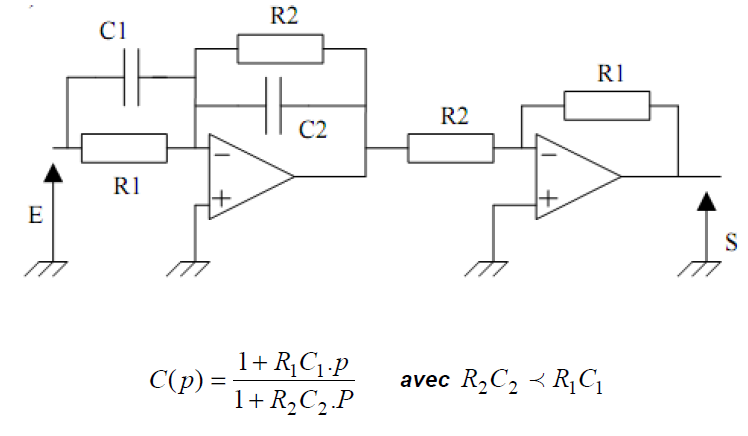
\includegraphics[width = 15cm]{Avph/Avph.png} 
\end{center}

\vspace{0.5cm}

Dans ce schémas, le produit $R_1*C_1$ correspond à la constante $ T_av$ définie dans le rapport d'automatique et le produit $R_2*C_2$ correspond à $0.1*T_av$.


Nous allons déterminer les valeurs de $R_1$, $R_2$, $C_1$ et $C_2$ dans deux configurations : poids du mobile à $0.0897 kg$ correspondant à un $T_av$ de 0.0313 et poids du mobile à $0.1414 kg$ correspondant à un $T_av$ de 0.0393.


Aussi, par le biais de MATLAB, nous avons pu obtenir la courbe théorique de notre correcteur par avance de phase :

\begin{center}
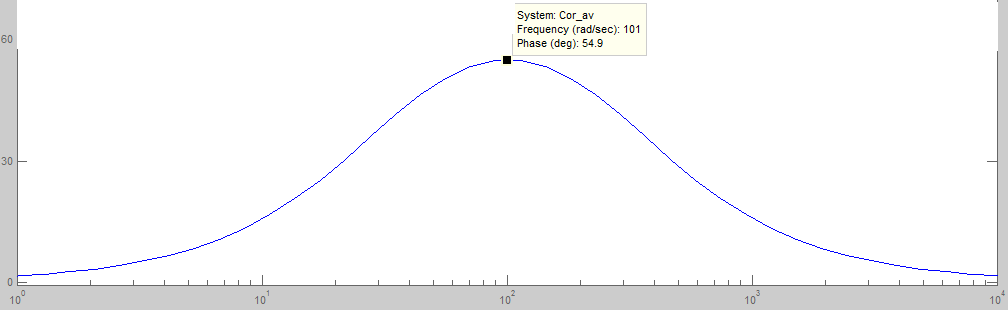
\includegraphics[width = 15cm]{Avph/aphmat.png} 
\end{center}

A noter que la fréquence donnée est en $rad.s^-1$, elle vaut environ 16Hz. 
\section{Détermination de valeurs des composants}

Pour des raisons de simplifications, nous prendrons les résistances $R_1$ et $R_2$ égales, le facteur 10 entre les constantes du numérateur et du dénominateur sera donc réalisé par un facteur 10 entre les valeurs des condensateurs. 



Pour le poids de $0.0897 kg$, en choisissant des composants avec des valeurs normalisées, on obtient $R=8.2 K\Omega$, $C_1=3.9 \mu F$ et $C_2=390 nF$. 



On fera plutôt varier les résistances que les condensateurs pour s'adapter au changement de poids. On conserve donc les mêmes valeurs de condensateurs. On trouve alors $R=10.076 K\Omega$. 



Il sera donc possible de prendre des potentiomètres pour ajuster les constantes, corrigeant ainsi les écards possibles des valeurs de condensateurs. 


\section{Validation par simulation PSpice}

On simule le correcteur à avance de phase par le schémas suivant : 

\begin{center}
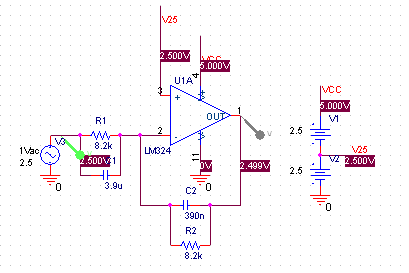
\includegraphics[width = 15cm]{Avph/schAvph.png} 
\end{center}

On obtient le résultat de simulation suivant : 

\begin{center}
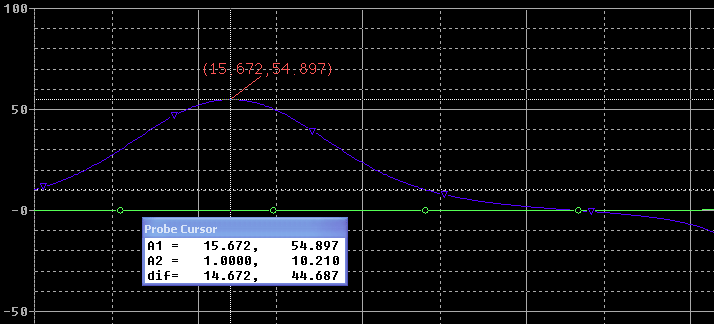
\includegraphics[width = 15cm]{Avph/simuAvph.png} 
\end{center}

Comme on peut le voir en comparant par rapport au résultat donné par MATLAB, le schéma répond comme on le souhaitait. 

\vspace{0.5cm}
\section{Conclusion}

\noindent
Nous avons donc validé notre choix de montage de correcteur et nous avons déterminer des valeurs admissibles de composants analogiques grâce à cette étude. Il faudra cependant être attentif quant au choix des condensateurs vis-à-vis de leur fréquence de fonctionnement.  

\pagebreak
\section{Bibliographie}

- Cours de GEE, A. Meghebbar :
\newline \textit{\underline{fsi.univ-tlemcen.dz/cours/Support-Cours-Commande-Analogique-Master-Electrotechnique10.pdf}}

\end{document}
